\documentclass{article}

\usepackage[dvipsnames]{xcolor}
\usepackage{graphicx}
\usepackage{amsmath}


\begin{document}

% Only use these colors for labels. 
\definecolor{cell_centered_color}{named}{Orange}
\definecolor{node_color}{named}{Red}
\definecolor{x_face_color}{named}{OliveGreen}
\definecolor{y_face_color}{named}{Blue}

\newcommand{\nodecolor}[1]{\textcolor{node_color}{#1}}
\newcommand{\cellcolor}[1]{\textcolor{cell_centered_color}{#1}}
\newcommand{\xfacecolor}[1]{\textcolor{x_face_color}{#1}}
\newcommand{\yfacecolor}[1]{\textcolor{y_face_color}{#1}}


\section{Governing Equaitons}
The shallow water equations are:

$$ \frac{\partial{\vec{V}}}{\partial t} + \eta \hat{N} \times P \vec{V} + \nabla \left( P + \frac{1}{2}\vec{V} \cdot \vec{V} \right) = 0$$

$$ \frac{\partial{P}}{\partial t} + \nabla \cdot \left( P \vec{V} \right) = 0$$

where:

$$ \eta = \frac{\nabla \times \vec{V}}{P} $$

Putting this in component form we get:


$$ { \frac{\partial u}{\partial t} }= \eta P v - \frac{\partial}{\partial x} \left( P + \frac{1}{2} (u^2 + v^2) \right)$$



$$  { \frac{\partial v}{\partial t} } = -\eta P u - \frac{\partial}{\partial y} \left( P + \frac{1}{2} (u^2 + v^2) \right)$$


$$  \frac{\partial P}{\partial t} = -\frac{\partial}{\partial x}\left(Pu\right) - \frac{\partial}{\partial y} (Pv) $$

$$ \eta = \frac{ \frac{\partial v}{\partial x} - \frac{\partial u}{\partial y} }{P} $$


\section{Domain}

%\includegraphics[width=\textwidth]{./figures/domain.png}

\begin{figure}[h!]
	%\includegraphics[width=\textwidth]{./figures/domain.png}
	\includegraphics[width=\textwidth]{./figures/Domain_Overview_With_Labels.jpg}
	\caption{Example Domain.}
	\label{fig: Domain}
\end{figure}

The equations are discretized on a two dimensional Cartesian domain $\Omega = \left\{ (x,y) : 0 \leq x \leq L_x,  0 \leq y \leq L_y \right\} $. The step size (dx, dy) and number of cells in each direction (Nx, Ny) can be varied independently. However typically the step size in each direction is kept at a default value of dx=dy=$10,000$. The user is given the option to change the number of cells (Nx, Ny) in each direction, which implicitly sets the length of the domain in each direction $(L_x = Nx * dx, L_y = Ny * dy)$.


\begin{figure}[h!]
	\includegraphics[width=\textwidth]{./figures/Unit_Cell_Cell_Centered.jpg}
	\caption{Variable Locations - Cell Centered View}
	\label{fig: Cell Centered Unit Cell}
\end{figure}

\begin{figure}[h!]
	\includegraphics[width=\textwidth]{./figures/Variable_Location_Color_Legend.png}
	\caption{Variable Locations Legend}
	\label{fig: Variable Location Legend}
\end{figure}


Figures \ref{fig: Cell Centered Unit Cell} and \ref{fig: Variable Location Legend} show where the variables are saved on the mesh. The indexing scheme used for the nodal, face centered, and cell centered values may vary depending on the implementation. The indexing scheme shown in \ref{fig: Cell Centered Unit Cell} is used in the AMReX versions of the mini-app. Note that the user inputs the number of cells in each direction (Nx, Ny), hence the data structures used to store values at the nodal and face centered locations need to be allocated larger to accommodate the extra values.  

\section{Initial Condition}
An analytical initial condition is specified the velocity and pressure.

The velocity is initialized using an analytical stream function. 

$$ \psi = A \sin(\xi_x) \sin(\xi_y) $$
where the amplitude is set to a default value of 
$$ A = 10^6 $$
and $\xi_x$ and $\xi_y$ are the spacial variables $x$ and $y$ transformed onto the interval $(0, 2\pi)$.
$$\xi_x = \frac{2\pi}{L_x}x$$
$$\xi_y = \frac{2\pi}{L_y}x$$

Then the initial velocity is set to:

$$ u_0 = -\frac{\partial \psi}{\partial y} $$
$$ v_0 = \frac{\partial \psi}{\partial x} $$

{\color{red}{Note: This is what is in the code but usually I see the stream function defined so that $u = \frac{\partial \phi}{\partial y}$ and $v = -\frac{\partial \phi}{\partial x}$}. I don't think it matters since either definition of the stream function automatically satisfies the two dimensional incompressible continuity equation. Just a note this is what most textbooks I have come across would call $-\psi$}

In the implementation the stream function $\psi$ is evaluated and saved at the cell centers, then the central finite difference is used to find $u$ and $v$ at the adjacent faces.


The initial pressure evaluated at all the nodal points using:
$$ P_0 =  \frac{\pi^2 A^2}{L_x^2} \left[ \cos(2 \xi_x) + \cos(2 \xi_y) \right] + 5000 $$ 




\section{Numerical Methods}

\section{Boundary Conditions}

\section{user Input}



\section{Labels}
This section was used to print symbols in large fonts so they could be copy pasted into presentations.

\begin{Huge}
	
	Legend:
	\begin{tabular}{ c l }
		\color{cell_centered_color}{$\bullet$} & \color{cell_centered_color}{Cell Centered} \\ 
		\color{node_color}{$\bullet$} & \color{node_color}{Node} \\  
		\color{x_face_color}{$\bullet$} & \color{x_face_color}{X Face} \\
		\color{y_face_color}{$\bullet$} & \color{y_face_color}{Y Face} 
	\end{tabular}
	
	\begin{tabular}{ c l }
	\color{cell_centered_color}{} & \color{cell_centered_color}{Cell Centered} \\ 
	\color{node_color}{} & \color{node_color}{Node} \\  
	\color{x_face_color}{} & \color{x_face_color}{X Face} \\
	\color{y_face_color}{} & \color{y_face_color}{Y Face} 
\end{tabular}	
	
 	\vspace{1in}
	Cell Center Values:
	\color{cell_centered_color}{ 
		$$ \psi_{i,j} $$ 
		$$ \psi_{i+1,j} $$
		$$ \psi_{i,j+1} $$
		$$ \psi_{i+1,j+1} $$ 
		$$ \psi_{i-1,j} $$ 
		$$ \psi_{i,j-1} $$
		$$ \psi_{i-1,j-1} $$
		
		$$ \eta_{i,j}$$
		
		$$ z $$
	}
	
	\color{node_color}{ 
		$$ p_{i,j} $$ 
		$$ p_{i+1,j} $$ 
		$$ p_{i,j+1} $$
		$$ p_{i+1,j+1} $$ 
		
		$$ h $$
		$$ h_{i,j} $$
	}
	
	
	\color{y_face_color}{ 
		$$ u_{i,j} $$ 
		$$ u_{i,j+1} $$ 
		$$ u_{i-1,j} $$ 		
		
		$$ cu $$
	}
	
	
	\color{x_face_color}{ 
		$$ v_{i,j} $$ 
		$$ v_{i+1,j} $$ 
		$$ v_{i,j-1} $$ 
				
		$$ cv $$
	}
	
	\color{black}{
	Initial Conditions:
	$$\vec{V}_0$$
	$$P_0$$
	
	Mesh: \\
	Nx \\
	Ny \\
	dx \\
	dy \\
	dx = dy = 10,000 \\
	N$_\mathrm{ghost}$ = 1 \\
	N$_\mathrm{grow}$ = 1 \\
	$L_x$ \\
	$L_y$ \\
	}
	
	
	
\end{Huge}

The shallow water equations are:
$$ \frac{\partial{\vec{V}}}{\partial t} + \eta \hat{N} \times P \vec{V} + \nabla \left( P + \frac{1}{2}\vec{V} \cdot \vec{V} \right) = 0$$

$$ \frac{\partial{P}}{\partial t} + \nabla \cdot \left( P \vec{V} \right) = 0$$

where:

$$ \eta = \frac{\nabla \times \vec{V}}{P} $$

Where in component form we get:


$$ \textcolor{y_face_color}{ \frac{\partial u}{\partial t} }= \eta P v - \frac{\partial}{\partial x} \left( P + \frac{1}{2} (u^2 + v^2) \right)$$



$$  \textcolor{x_face_color}{ \frac{\partial v}{\partial t} } = -\eta P u - \frac{\partial}{\partial y} \left( P + \frac{1}{2} (u^2 + v^2) \right)$$


$$ \nodecolor{ \frac{\partial P}{\partial t} } = -\frac{\partial}{\partial x}\left(Pu\right) - \frac{\partial}{\partial y} (Pv) $$

$$ \textcolor{cell_centered_color}{\eta} = \frac{ \frac{\partial v}{\partial x} - \frac{\partial u}{\partial y} }{P} $$

$$ \textcolor{node_color}{h_{i,j}} = \textcolor{node_color}{P_{i,j}} + \frac{1}{2} \left( \frac{\textcolor{y_face_color}{u_{i-1,j}}^2 + \textcolor{y_face_color}{u_{i,j}}^2}{2} + \frac{\textcolor{x_face_color}{v_{i,j-1}}^2 + \textcolor{x_face_color}{v_{i,j}}^2}{2} \right) $$


$$ \textcolor{y_face_color}{[Pu]_{i,j}}  = \frac{ \textcolor{node_color}{P_{i,j}} + \textcolor{node_color}{P_{i+1,j}} }{2} \textcolor{y_face_color}{u_{i,j}} $$


$$ \textcolor{x_face_color}{[Pv]_{i,j}} = \frac{\textcolor{node_color}{P_{i,j}} + \textcolor{node_color}{P_{i,j+1}}}{2} \textcolor{x_face_color}{v_{i,j}}$$

$$ \textcolor{cell_centered_color}{\eta_{i,j}} = \frac{ \frac{ \textcolor{x_face_color}{v_{i+1,j}} - \textcolor{x_face_color}{v_{i,j}}}{dx} - \frac{ \textcolor{y_face_color}{u_{i,j+1}} - \textcolor{y_face_color}{u_{i,j}} }{dy} }{\frac{ \textcolor{node_color}{P_{i,j}} + \textcolor{node_color}{P_{i+1,j}} + \textcolor{node_color}{P_{i,j+1}} + \textcolor{node_color}{P_{i+1,j+1}} }{4} } $$

$$ \frac{\partial \yfacecolor{u_{i,j}}}{\partial t} = \left( \frac{ \cellcolor{\eta_{i,j-1}} + \cellcolor{\eta_{i,j}} }{2} \right) \left( \frac{ \xfacecolor{[P v]_{i,j-1}} + \xfacecolor{[P v]_{i,j}} + \xfacecolor{[P v]_{i+1,j-1}} + \xfacecolor{[P v]_{i+1,j}} }{4} \right) - \left(\frac{ \nodecolor{ h_{i+1,j} } -  \nodecolor{ h_{i,j} } }{dx} \right)  $$

$$ \frac{\partial \xfacecolor{v_{i,j}}}{\partial t} = \left( \frac{ \textcolor{cell_centered_color}{\eta_{i-1,j}} +  \textcolor{cell_centered_color}{\eta_{i,j}} }{2} \right) \left( \frac{ \yfacecolor{[P u]_{i-1,j}} + \yfacecolor{[P u]_{i-1,j+1}} + \yfacecolor{[P u]_{i,j}} + \yfacecolor{[P u]_{i,j+1}} }{4} \right) - \left( \frac{ \nodecolor{h_{i,j+1}} - \nodecolor{h_{i,j}} }{dy} \right)  $$

$$ \frac{\partial \nodecolor{P_{i,j}}}{\partial t} = - \left( \frac{ \yfacecolor{[Pu]_{i,j}} - \yfacecolor{[Pu]_{i-1,j}} }{dx} \right) - \left(  \frac{ \xfacecolor{[Pv]_{i,j}} - \xfacecolor{[Pu]_{i,j-1}}}{dy} \right) $$

\section{Governing Equations to Reduce the Memory Footprint}

Plug the potential vorticity into the governing equations for momentum.

$$ \textcolor{y_face_color}{ \frac{\partial u}{\partial t} }= \left( \frac{\partial v}{\partial x} - \frac{\partial u}{\partial y} \right) v - \frac{\partial}{\partial x} \left( P + \frac{1}{2} (u^2 + v^2) \right)$$


$$  \textcolor{x_face_color}{ \frac{\partial v}{\partial t} } = \left( \frac{\partial v}{\partial x} - \frac{\partial u}{\partial y} \right) u - \frac{\partial}{\partial y} \left( P + \frac{1}{2} (u^2 + v^2) \right)$$


$$ \nodecolor{ \frac{\partial P}{\partial t} } = -\frac{\partial}{\partial x}\left(Pu\right) - \frac{\partial}{\partial y} (Pv) $$


\subsection{Equations for interpolating from one location to another}

X\_face to node
%$$ \nodecolor{\phi_{i,j}} = \frac{\xfacecolor{\phi_{i,j-1}} + \xfacecolor{\phi_{i,j}} } {2} $$
%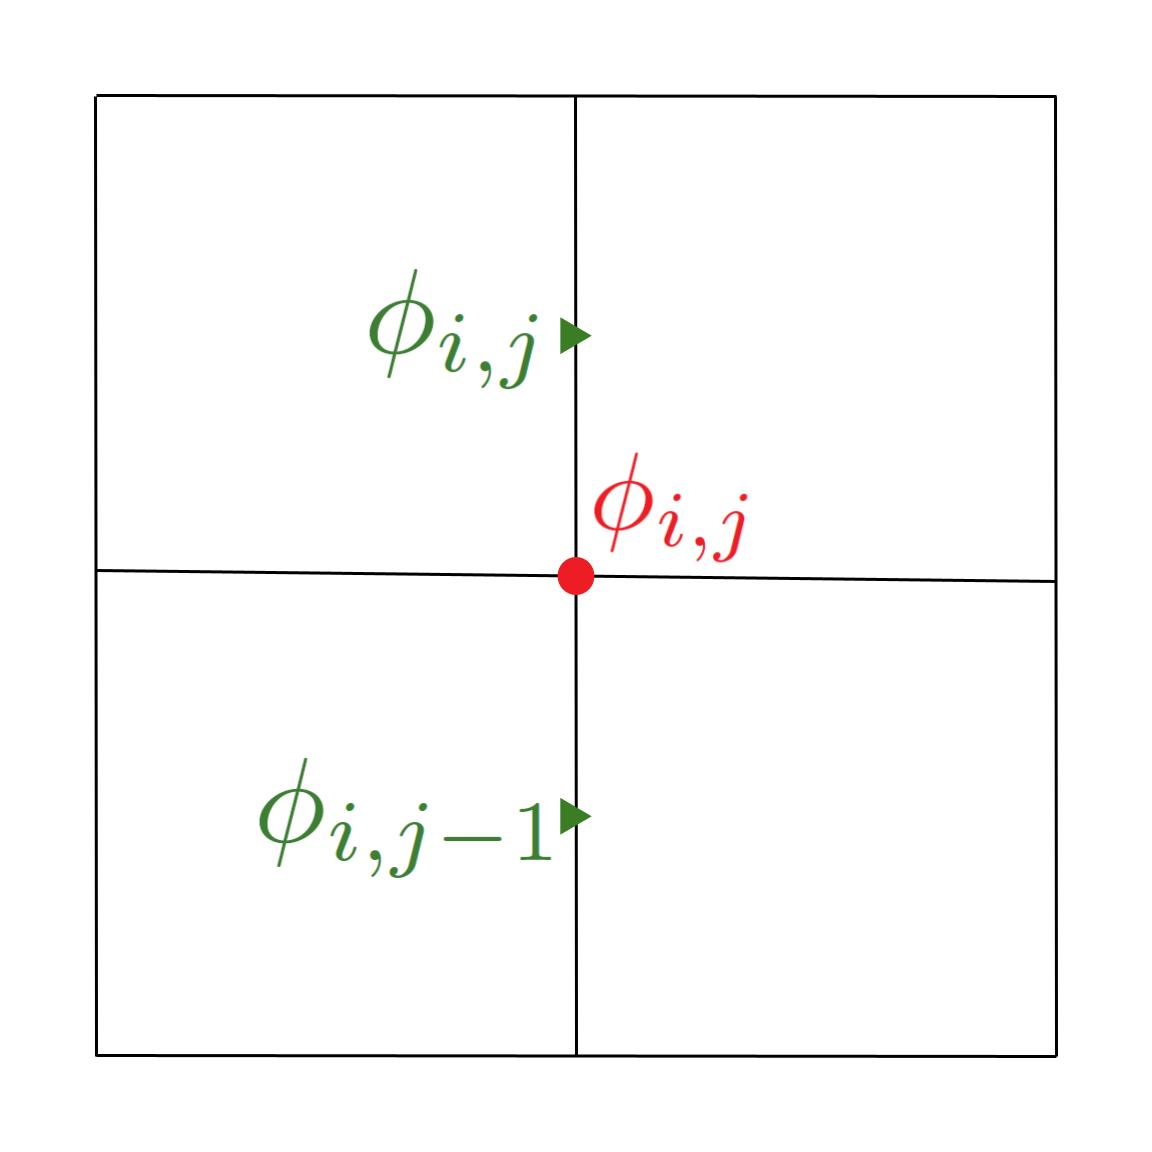
\includegraphics[width=0.5\textwidth]{./figures/interpolate/Interpolate_X_Face_to_Node.jpg}


\begin{center}
	\begin{minipage}[c]{0.45\textwidth} % 45% of the page width
		\Large
		\begin{equation*}
			\nodecolor{\phi_{i,j}} = \frac{\xfacecolor{\phi_{i,j-1}} + \xfacecolor{\phi_{i,j}} }{2}
		\end{equation*}
	\end{minipage}
	\hfill % Horizontal space between the two minipages
	\begin{minipage}[c]{0.45\textwidth} % 45% of the page width
		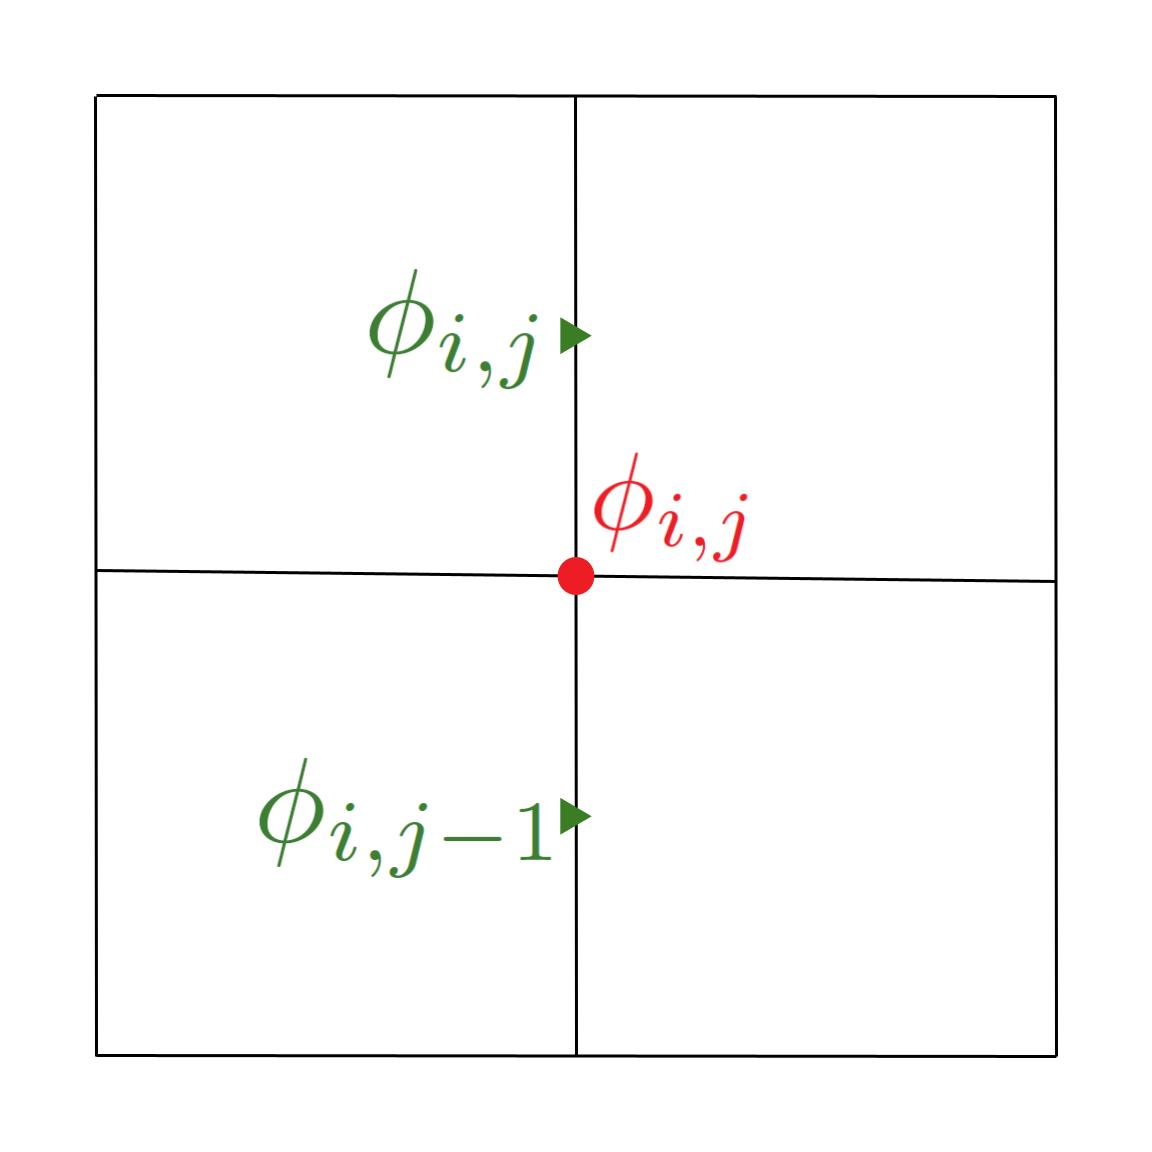
\includegraphics[width=\textwidth]{./figures/interpolate/Interpolate_X_Face_to_Node.jpg} % Replace 'example-image' with your image file
	\end{minipage}
\end{center}


X\_face to Y\_face
%$$ \yfacecolor{\phi_{i,j}} = \frac{\xfacecolor{\phi_{i,j-1}} + \xfacecolor{\phi_{i+1,j-1}} + \xfacecolor{\phi_{i,j}} + \xfacecolor{\phi_{i+1,j}} } {4} $$

\begin{center}
	\begin{minipage}[c]{0.45\textwidth} % 45% of the page width
		\begin{equation*}
			\yfacecolor{\phi_{i,j}} = \frac{\xfacecolor{\phi_{i,j-1}} + \xfacecolor{\phi_{i+1,j-1}} + \xfacecolor{\phi_{i,j}} + \xfacecolor{\phi_{i+1,j}} } {4}
		\end{equation*}
	\end{minipage}
	\hfill % Horizontal space between the two minipages
	\begin{minipage}[c]{0.45\textwidth} % 45% of the page width
		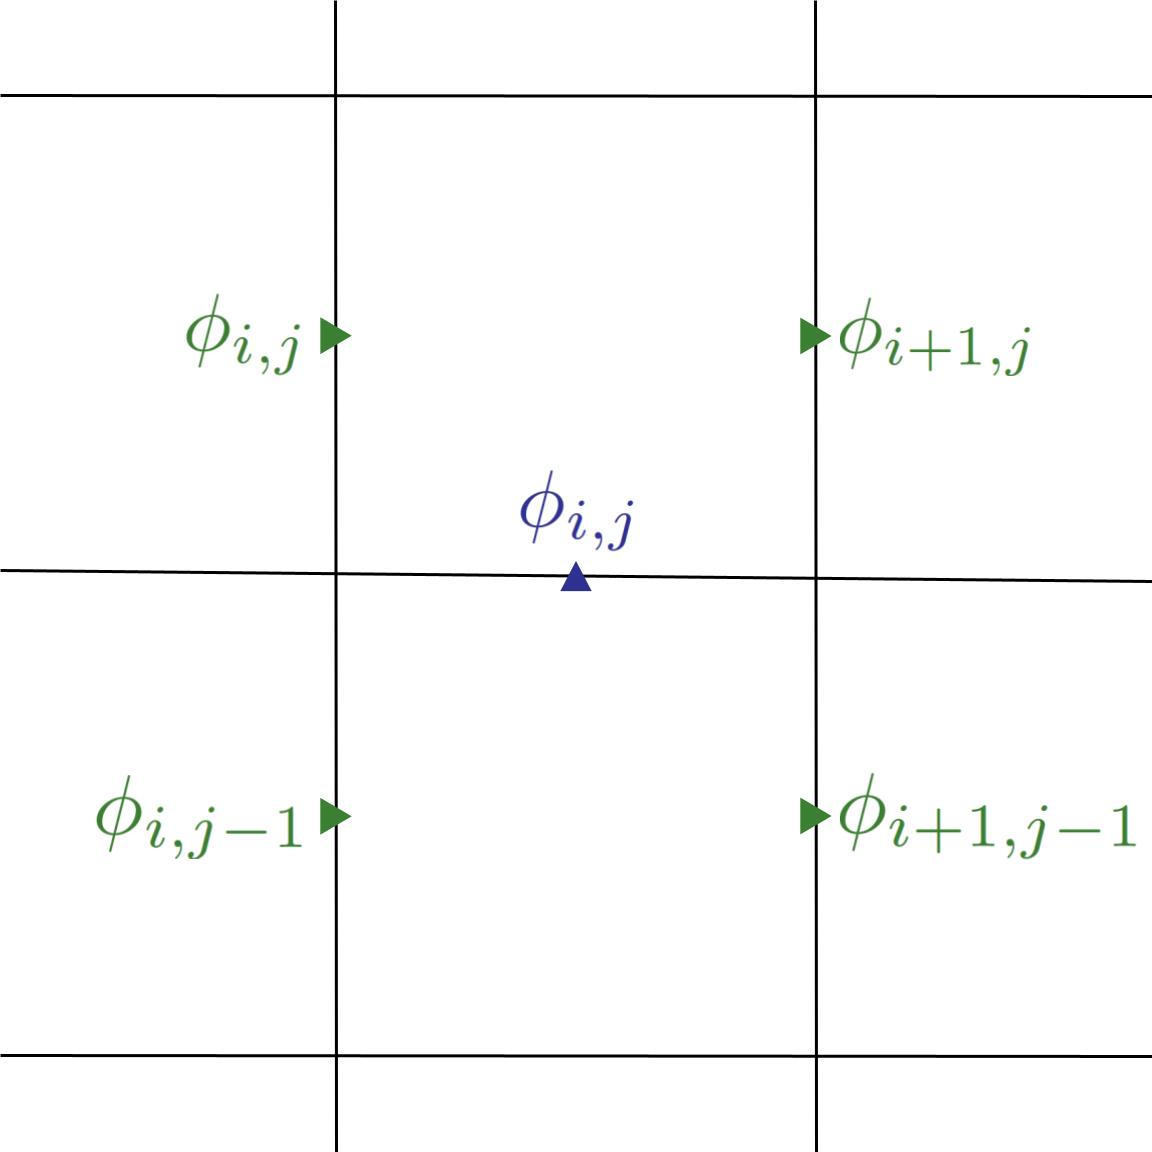
\includegraphics[width=\textwidth]{./figures/interpolate/Interpolate_X_Face_to_Y_Face.jpg} % Replace 'example-image' with your image file
	\end{minipage}
\end{center}

X\_face to cell center
%$$ \cellcolor{\phi_{i,j}} = \frac{\xfacecolor{\phi_{i,j}} + \xfacecolor{\phi_{i+1,j}} } {2} $$

\begin{center}
	\begin{minipage}[c]{0.45\textwidth} % 45% of the page width
		\Large
		\begin{equation*}
			\cellcolor{\phi_{i,j}} = \frac{\xfacecolor{\phi_{i,j}} + \xfacecolor{\phi_{i+1,j}} } {2}
		\end{equation*}
	\end{minipage}
	\hfill % Horizontal space between the two minipages
	\begin{minipage}[c]{0.45\textwidth} % 45% of the page width
		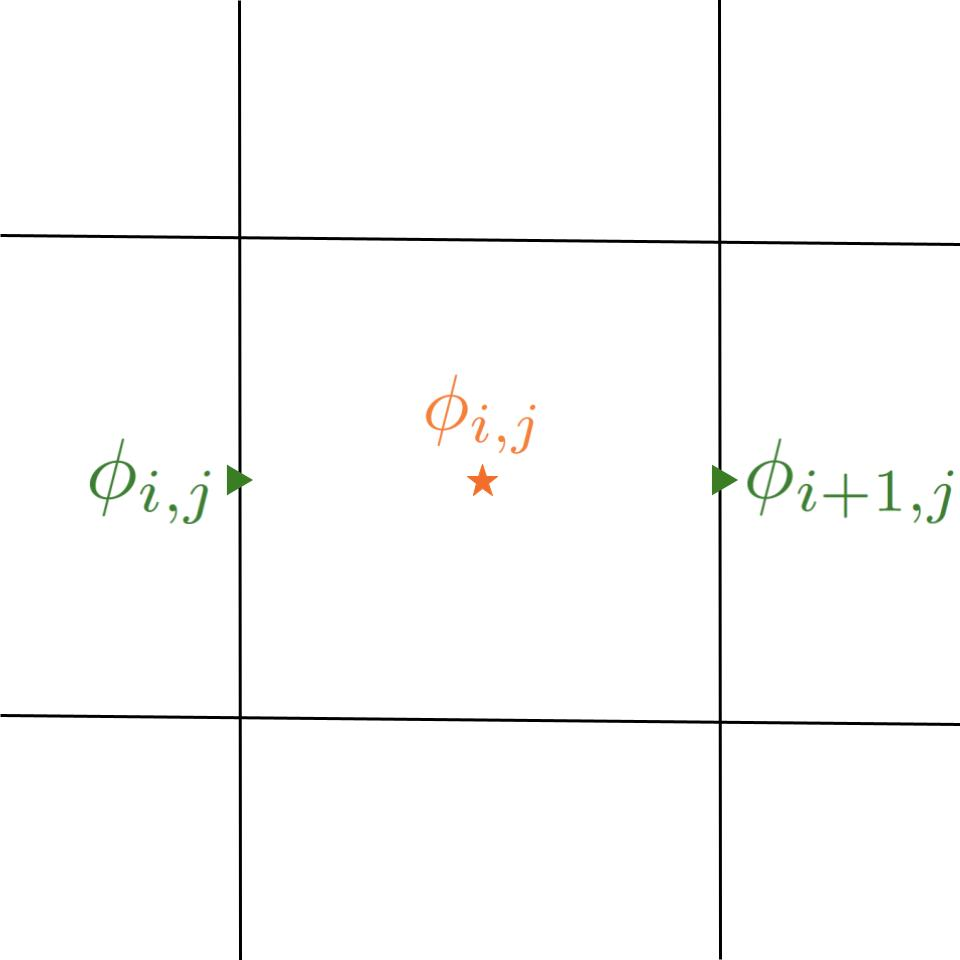
\includegraphics[width=\textwidth]{./figures/interpolate/Interpolate_X_Face_to_Cell_Center.jpg} % Replace 'example-image' with your image file
	\end{minipage}
\end{center}

Y\_face to node
%$$ \nodecolor{\phi_{i,j}} = \frac{\yfacecolor{\phi_{i-1,j}} + \yfacecolor{\phi_{i,j}} } {2} $$

\begin{center}
	\begin{minipage}[c]{0.45\textwidth} % 45% of the page width
		\Large
		\begin{equation*}
			\nodecolor{\phi_{i,j}} = \frac{\yfacecolor{\phi_{i-1,j}} + \yfacecolor{\phi_{i,j}} } {2}
		\end{equation*}
	\end{minipage}
	\hfill 
	\begin{minipage}[c]{0.45\textwidth} 
		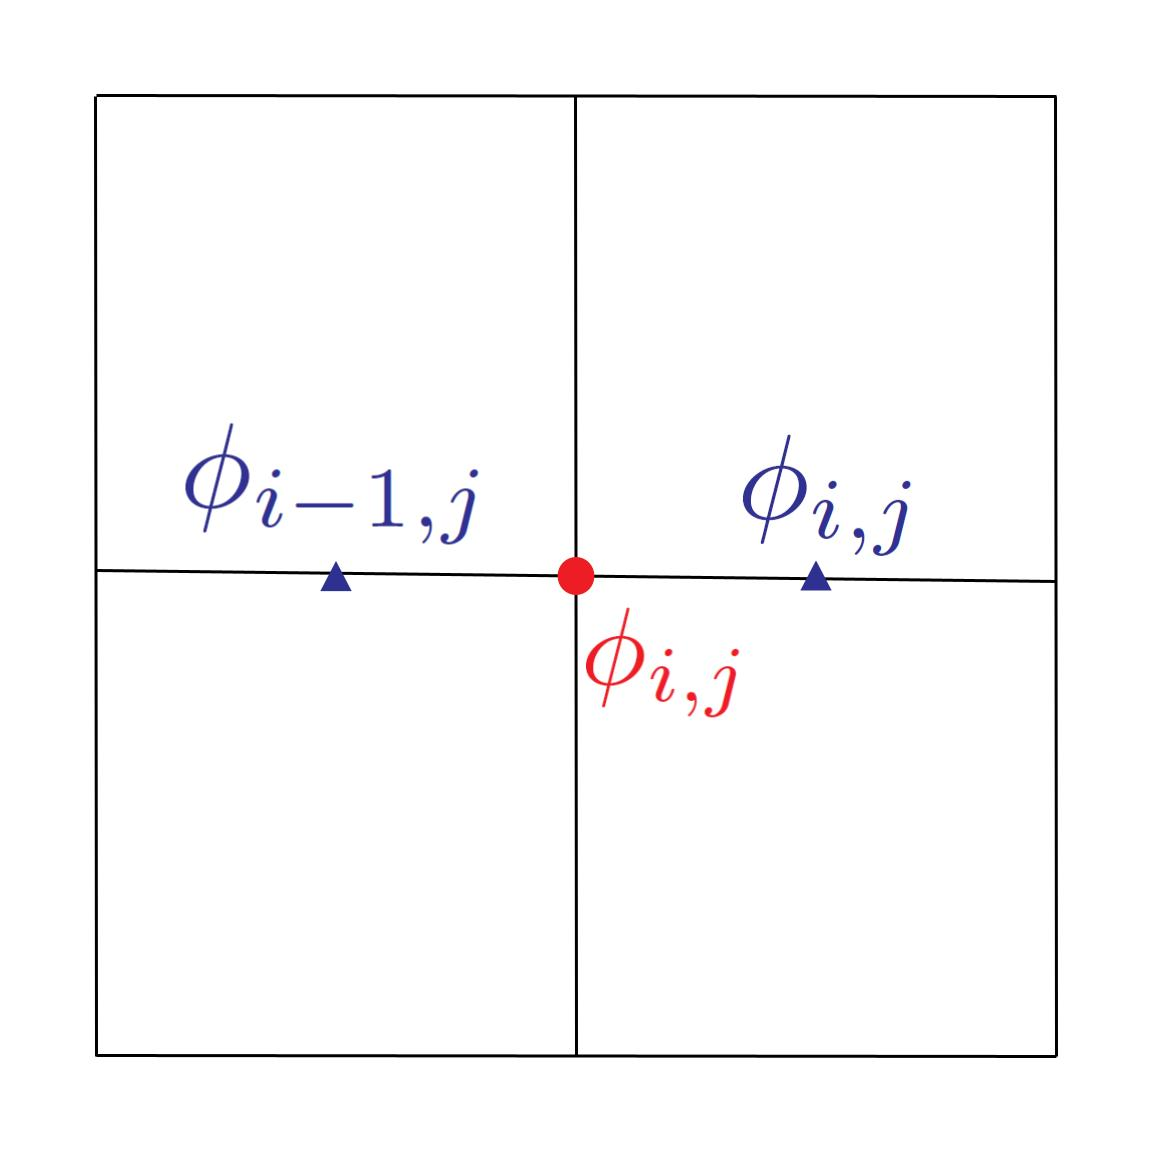
\includegraphics[width=\textwidth]{./figures/interpolate/Interpolate_Y_Face_to_Node.jpg}
	\end{minipage}
\end{center}

Y\_face to X\_face
%$$ \xfacecolor{\phi_{i,j}} = \frac{\yfacecolor{\phi_{i-1,j}} + \yfacecolor{\phi_{i,j}} + \yfacecolor{\phi_{i-1,j+1}} + \yfacecolor{\phi_{i,j+1}} } {4} $$

\begin{center}
	\begin{minipage}[c]{0.45\textwidth} % 45% of the page width
		\begin{equation*}
			\xfacecolor{\phi_{i,j}} = \frac{\yfacecolor{\phi_{i-1,j}} + \yfacecolor{\phi_{i,j}} + \yfacecolor{\phi_{i-1,j+1}} + \yfacecolor{\phi_{i,j+1}} } {4}
		\end{equation*}
	\end{minipage}
	\hfill 
	\begin{minipage}[c]{0.45\textwidth} 
		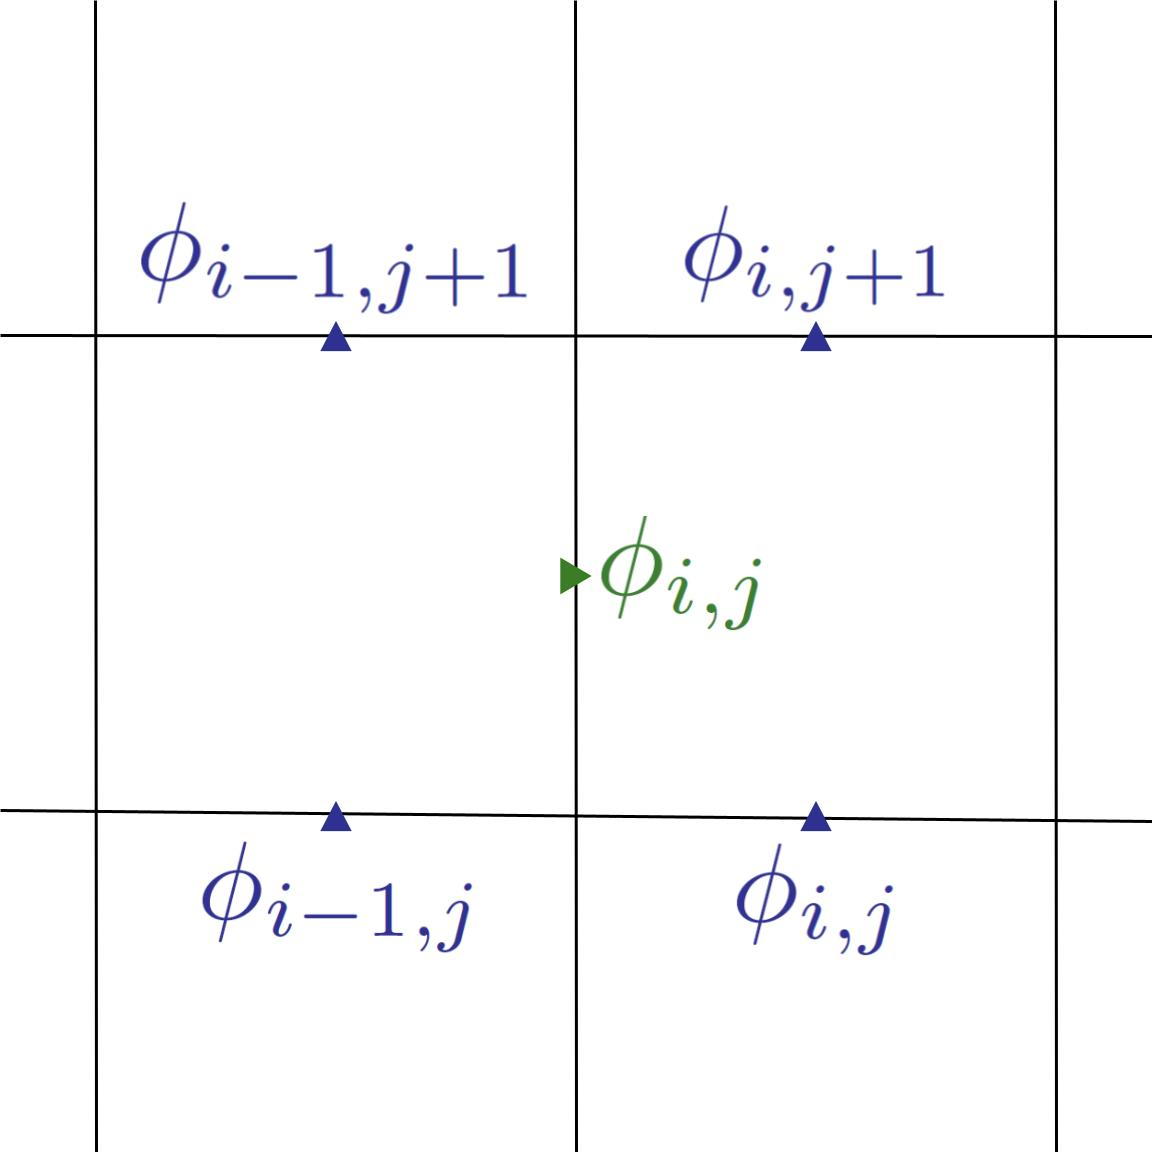
\includegraphics[width=\textwidth]{./figures/interpolate/Interpolate_Y_Face_to_X_Face.jpg}
	\end{minipage}
\end{center}

Y\_face to cell center
%$$ \cellcolor{\phi_{i,j}} = \frac{\yfacecolor{\phi_{i,j}} + \yfacecolor{\phi_{i,j+1}} } {2} $$

\begin{center}
	\begin{minipage}[c]{0.45\textwidth} % 45% of the page width
		\Large
		\begin{equation*}
			\cellcolor{\phi_{i,j}} = \frac{\yfacecolor{\phi_{i,j}} + \yfacecolor{\phi_{i,j+1}} } {2}
		\end{equation*}
	\end{minipage}
	\hfill 
	\begin{minipage}[c]{0.45\textwidth} 
		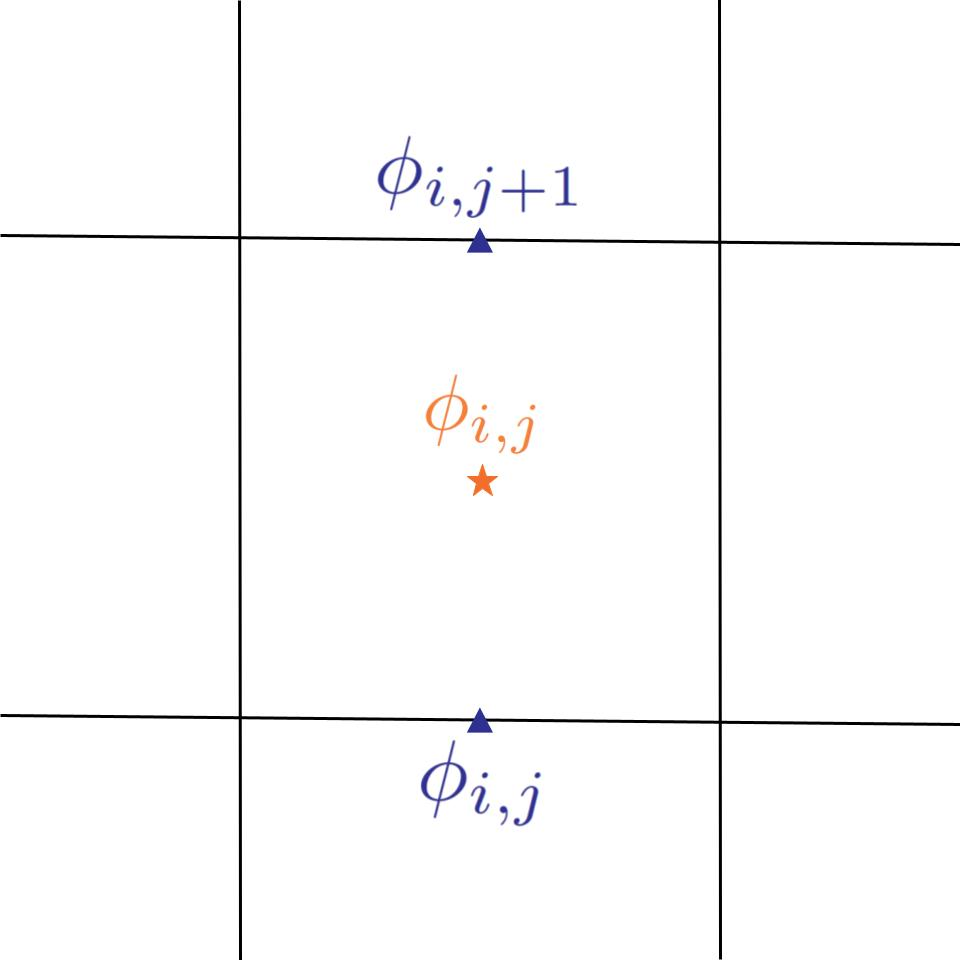
\includegraphics[width=\textwidth]{./figures/interpolate/Interpolate_Y_Face_to_Cell_Center.jpg}
	\end{minipage}
\end{center}

Node to X\_face
%$$ \xfacecolor{\phi_{i,j}} = \frac{ \nodecolor{\phi_{i,j}} + \nodecolor{\phi_{i,j+1}} } {2} $$

\begin{center}
	\begin{minipage}[c]{0.45\textwidth} % 45% of the page width
		\Large
		\begin{equation*}
			\xfacecolor{\phi_{i,j}} = \frac{ \nodecolor{\phi_{i,j}} + \nodecolor{\phi_{i,j+1}} } {2}
		\end{equation*}
	\end{minipage}
	\hfill 
	\begin{minipage}[c]{0.45\textwidth} 
		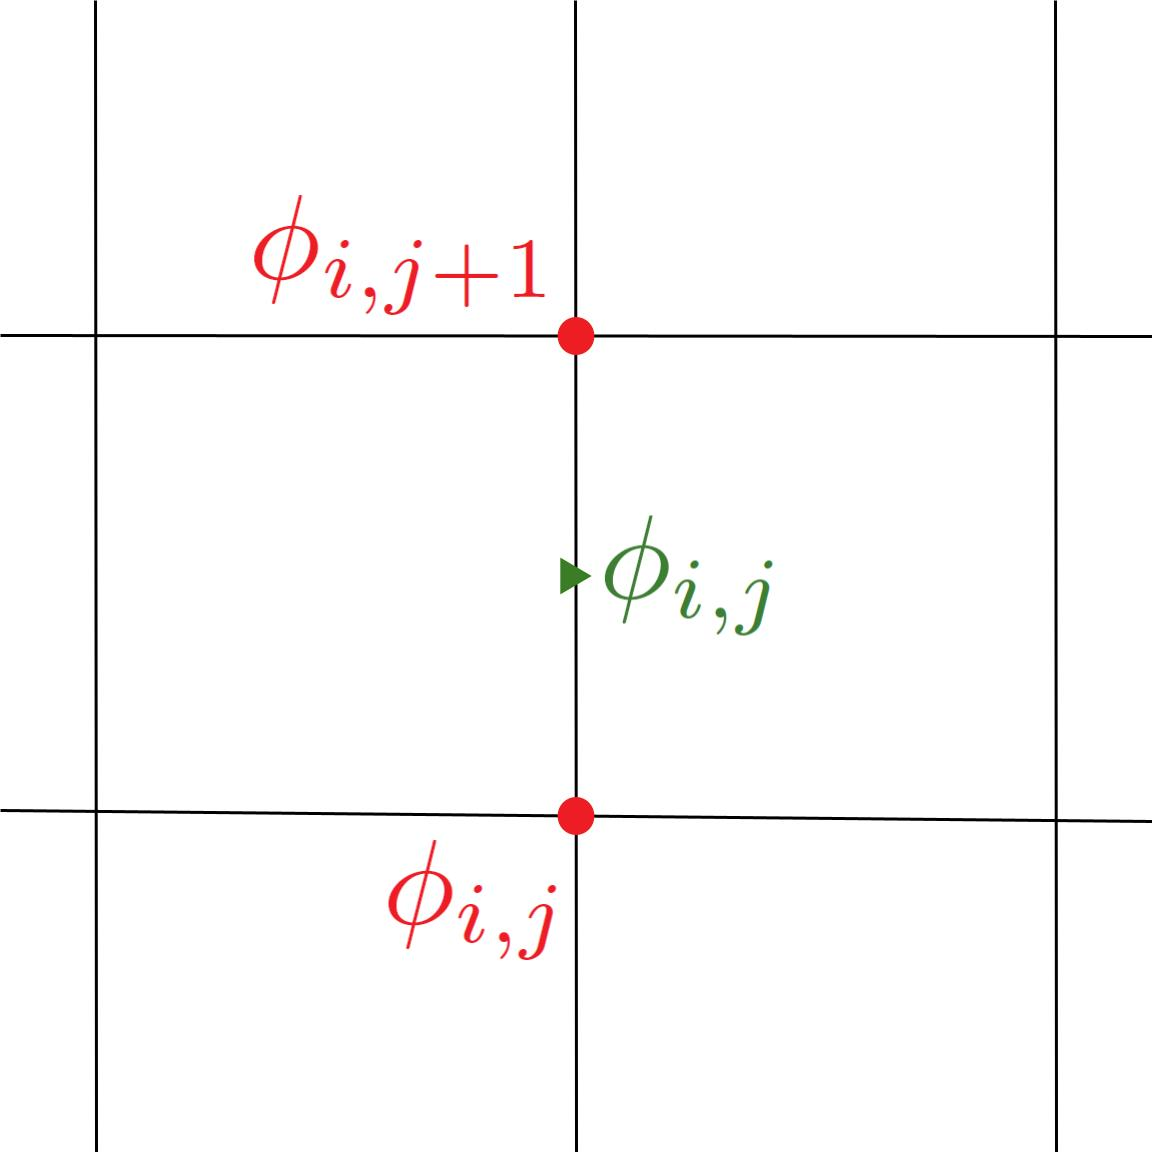
\includegraphics[width=\textwidth]{./figures/interpolate/Interpolate_Node_to_X_Face.jpg}
	\end{minipage}
\end{center}

Node to Y\_face
%$$ \yfacecolor{\phi_{i,j}} = \frac{ \nodecolor{\phi_{i,j}} + \nodecolor{\phi_{i+1,j}} } {2} $$

\begin{center}
	\begin{minipage}[c]{0.45\textwidth} % 45% of the page width
		\Large
		\begin{equation*}
			\yfacecolor{\phi_{i,j}} = \frac{ \nodecolor{\phi_{i,j}} + \nodecolor{\phi_{i+1,j}} } {2} 
		\end{equation*}
	\end{minipage}
	\hfill 
	\begin{minipage}[c]{0.45\textwidth} 
		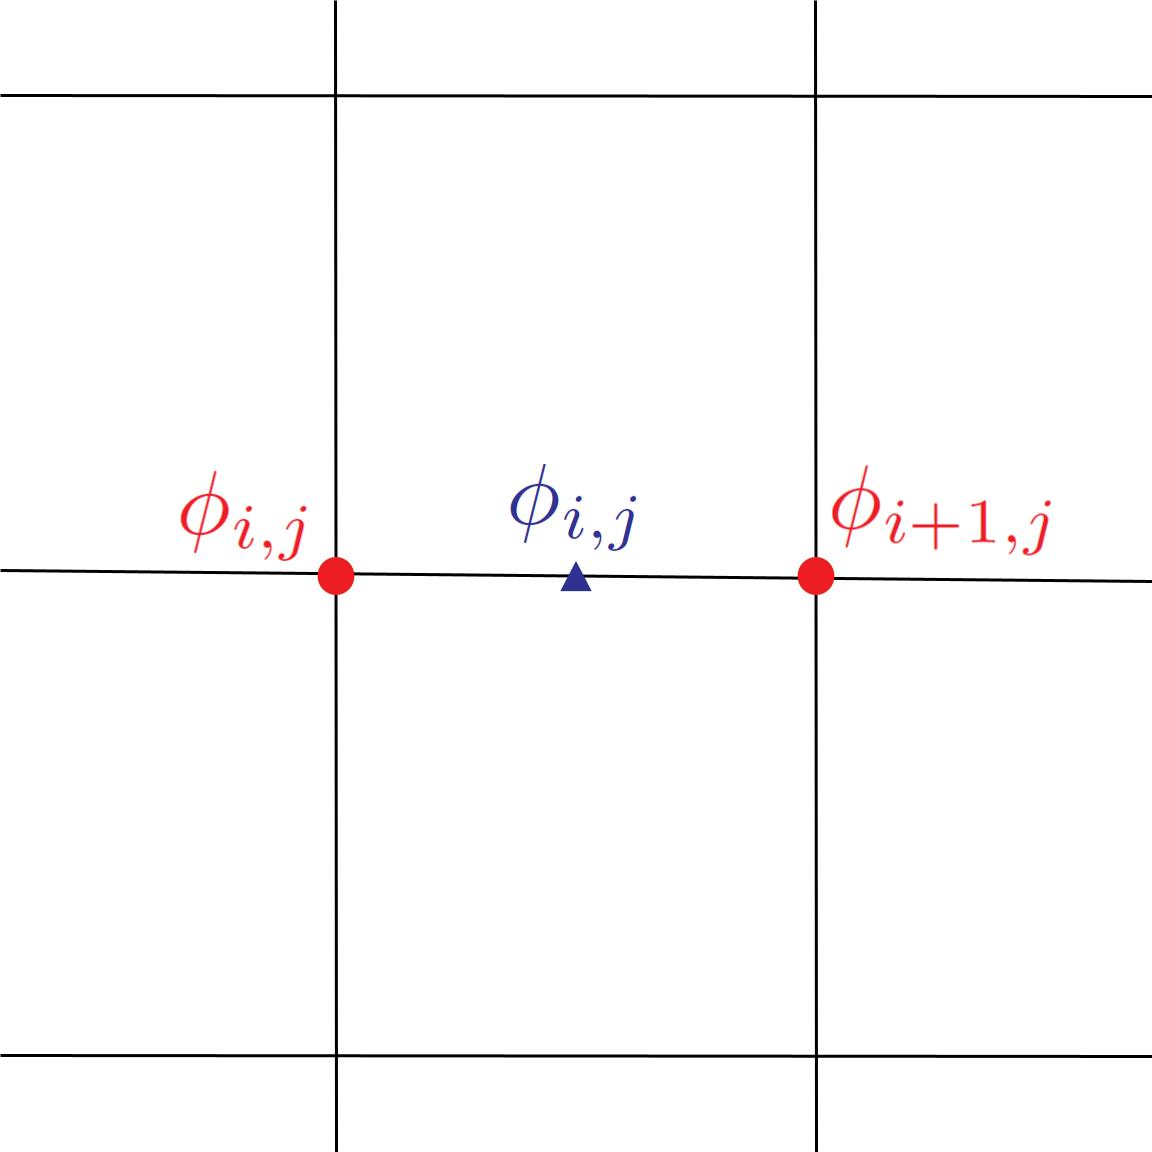
\includegraphics[width=\textwidth]{./figures/interpolate/Interpolate_Node_to_Y_Face.jpg}
	\end{minipage}
\end{center}

Node to cell center
%$$ \cellcolor{\phi_{i,j}} = \frac{ \nodecolor{\phi_{i,j}} + \nodecolor{\phi_{i+1,j}} + \nodecolor{\phi_{i,j+1}} + \nodecolor{\phi_{i+1,j+1}} } {4} $$

\begin{center}
	\begin{minipage}[c]{0.45\textwidth} % 45% of the page width
		\begin{equation*}
			\cellcolor{\phi_{i,j}} = \frac{ \nodecolor{\phi_{i,j}} + \nodecolor{\phi_{i+1,j}} + \nodecolor{\phi_{i,j+1}} + \nodecolor{\phi_{i+1,j+1}} } {4}
		\end{equation*}
	\end{minipage}
	\hfill 
	\begin{minipage}[c]{0.45\textwidth} 
		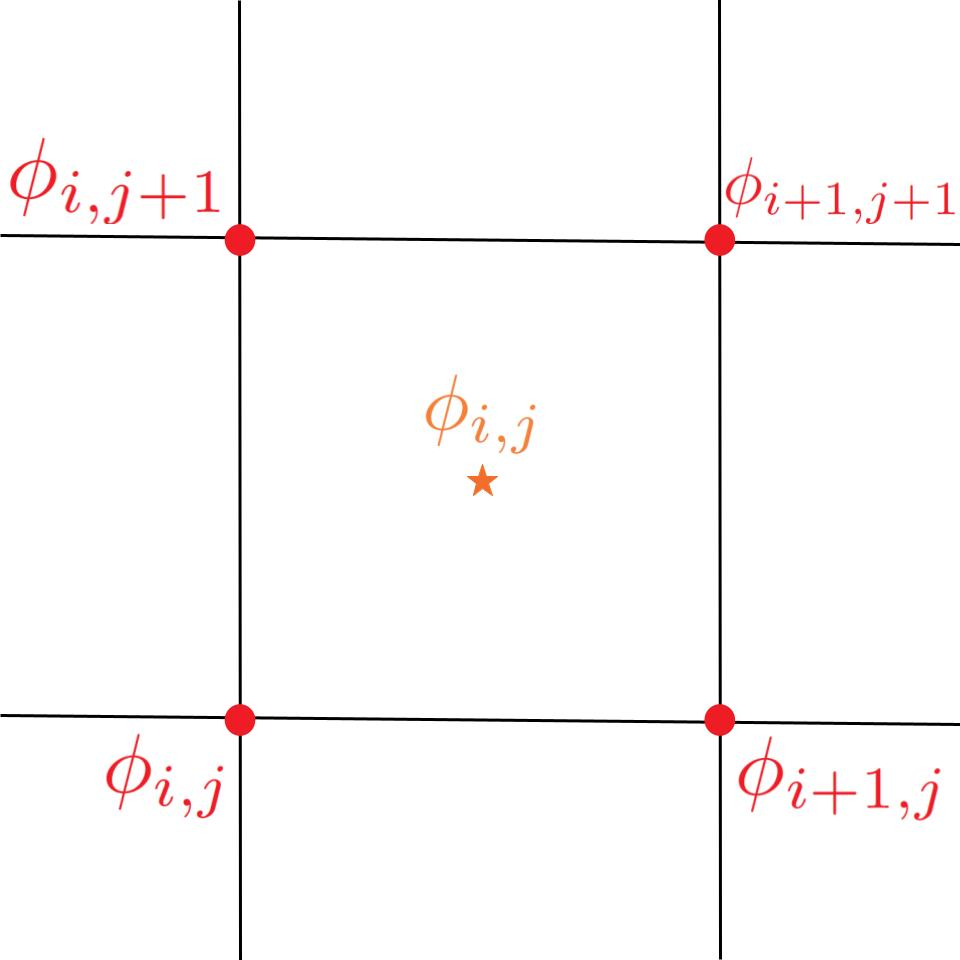
\includegraphics[width=\textwidth]{./figures/interpolate/Interpolate_Node_to_Cell_Center.jpg}
	\end{minipage}
\end{center}


Cell Center to X\_Face
%$$ \xfacecolor{\phi_{i,j}} = \frac{ \cellcolor{\phi_{i-1,j}} + \cellcolor{\phi_{i,j}} }{2} $$

\begin{center}
	\begin{minipage}[c]{0.45\textwidth} % 45% of the page width
		\Large
		\begin{equation*}
			\xfacecolor{\phi_{i,j}} = \frac{ \cellcolor{\phi_{i-1,j}} + \cellcolor{\phi_{i,j}} }{2}
		\end{equation*}
	\end{minipage}
	\hfill 
	\begin{minipage}[c]{0.45\textwidth} 
		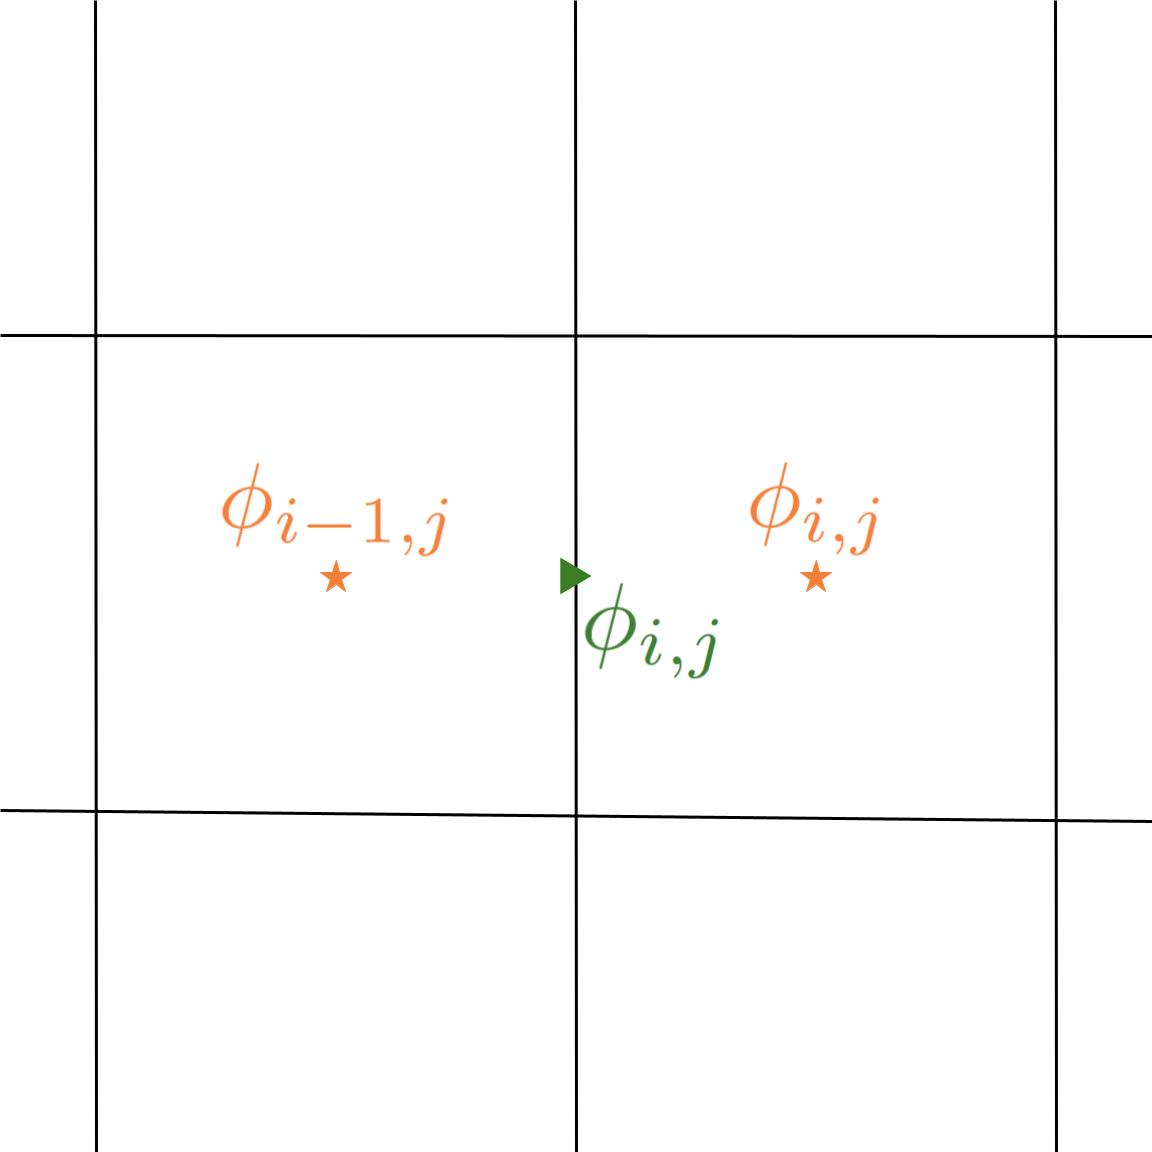
\includegraphics[width=\textwidth]{./figures/interpolate/Interpolate_Cell_Center_to_X_Face.jpg}
	\end{minipage}
\end{center}

Cell Center to Y\_Face
%$$ \yfacecolor{\phi_{i,j}} = \frac{ \cellcolor{\phi_{i,j-1}} + \cellcolor{\phi_{i,j}} }{2} $$

\begin{center}
	\begin{minipage}[c]{0.45\textwidth} % 45% of the page width
		\Large
		\begin{equation*}
			\yfacecolor{\phi_{i,j}} = \frac{ \cellcolor{\phi_{i,j-1}} + \cellcolor{\phi_{i,j}} }{2}
		\end{equation*}
	\end{minipage}
	\hfill 
	\begin{minipage}[c]{0.45\textwidth} 
		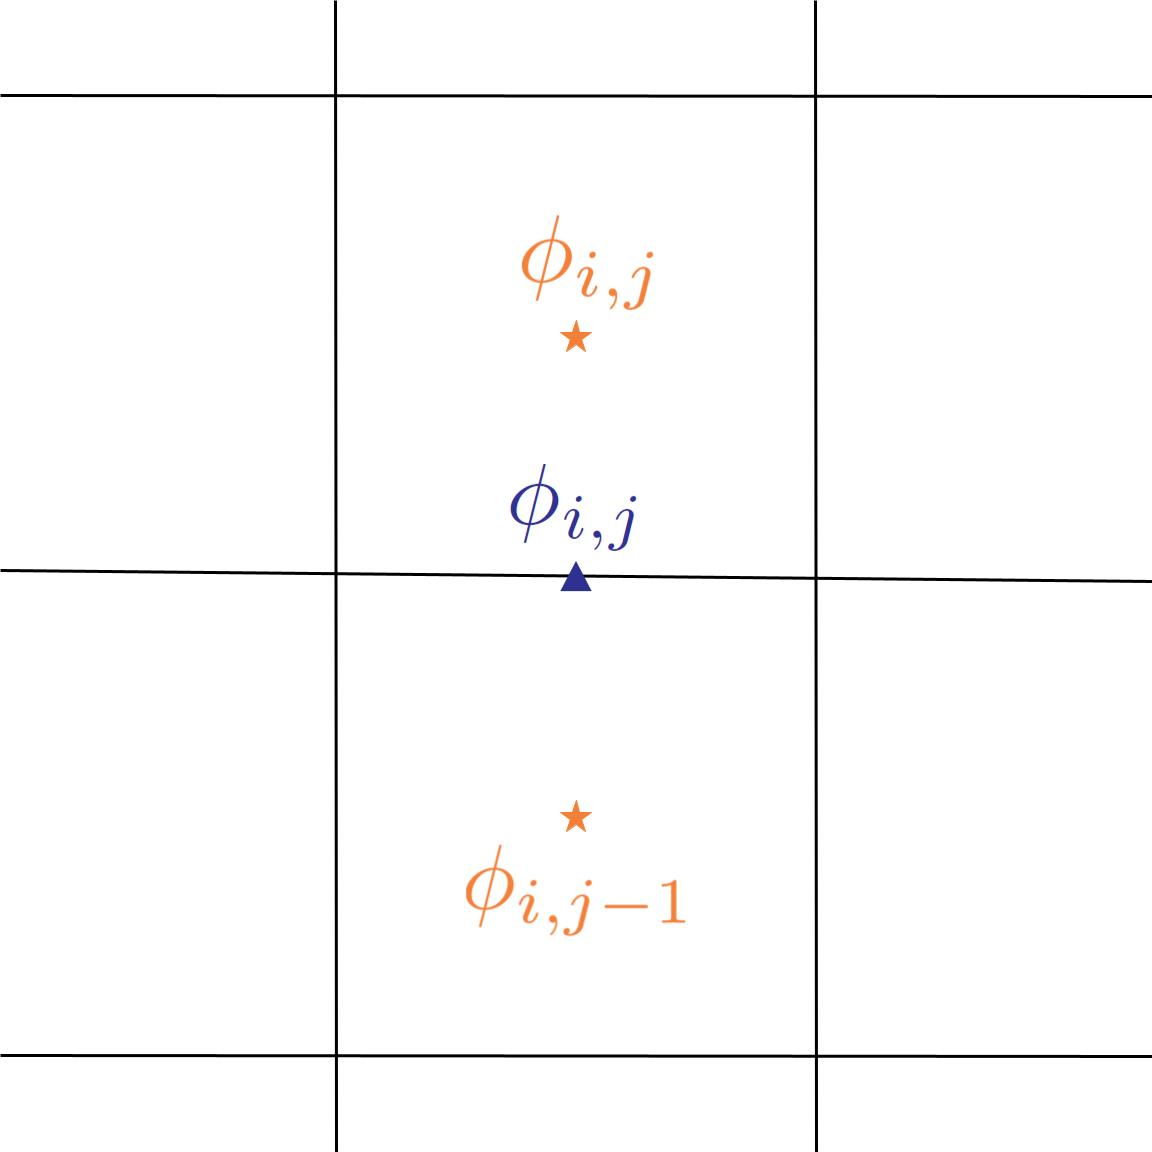
\includegraphics[width=\textwidth]{./figures/interpolate/Interpolate_Cell_Center_to_Y_Face.jpg}
	\end{minipage}
\end{center}

Cell Center to Node
%$$ \nodecolor{\phi_{i,j}} = \frac{ \cellcolor{\phi_{i-1,j-1}} + \cellcolor{\phi_{i-1,j}} + \cellcolor{\phi_{i,j-1}} + \cellcolor{\phi_{i,j}} }{4} $$

\begin{center}
	\begin{minipage}[c]{0.45\textwidth} % 45% of the page width
		\begin{equation*}
			\nodecolor{\phi_{i,j}} = \frac{ \cellcolor{\phi_{i-1,j-1}} + \cellcolor{\phi_{i-1,j}} + \cellcolor{\phi_{i,j-1}} + \cellcolor{\phi_{i,j}} }{4}
		\end{equation*}
	\end{minipage}
	\hfill 
	\begin{minipage}[c]{0.45\textwidth} 
		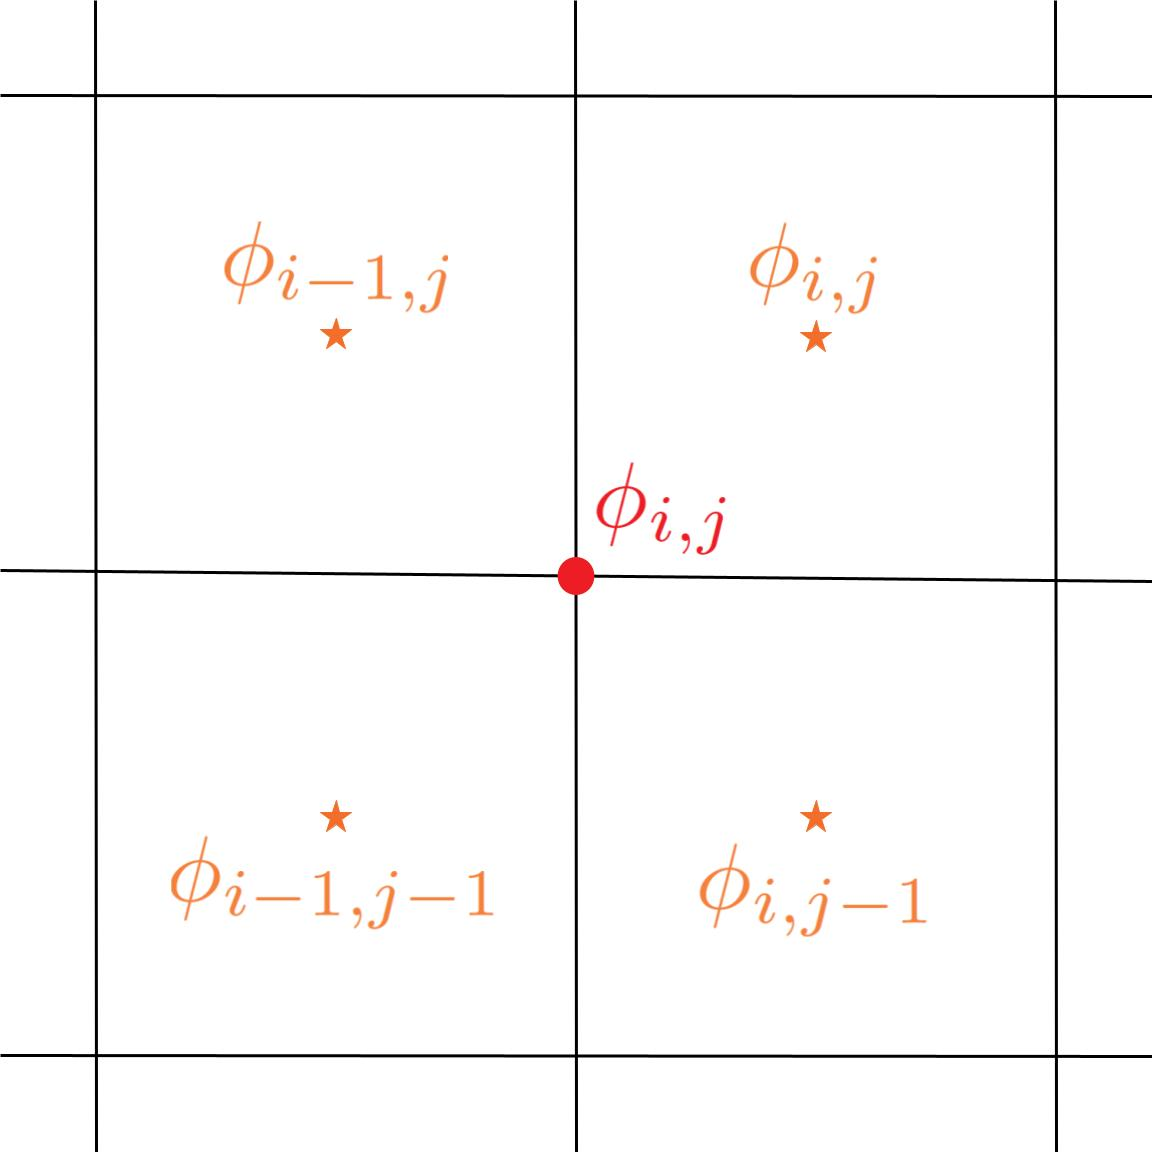
\includegraphics[width=\textwidth]{./figures/interpolate/Interpolate_Cell_Center_to_Node.jpg}
	\end{minipage}
\end{center}

\end{document}